\documentclass[12pt,a4paper]{article}

% ---------- Packages ----------
\usepackage[a4paper,margin=1in]{geometry}
\usepackage{graphicx}
\usepackage{setspace}
\usepackage{titlesec}
\usepackage{array}
\usepackage{tabularx}
\usepackage{lmodern}
\usepackage[T1]{fontenc}
\usepackage{hyperref}
\usepackage{float}     % enables [H] to place figures exactly "HERE"
\usepackage{placeins}  % provides \FloatBarrier to stop floats moving past a point
\hypersetup{colorlinks=true, linkcolor=black, urlcolor=black}

% ---------- Colors (optional subtle accent) ----------
\usepackage{xcolor}
\definecolor{SUblue}{RGB}{0,51,102} % Sabancı-style deep blue

% ---------- Titlepage ----------
\begin{document}
\thispagestyle{empty}
\begin{titlepage}
    \centering

    % --- University Name ---
    {\Large\bfseries \textcolor{SUblue}{Sabancı University}}\par
    \vspace{0.15cm}
    {\large Faculty of Engineering and Natural Sciences}\par
    \vspace{1.2cm}

    % --- Course Block ---
    {\large \textbf{ENS491 — Graduation Project Case Study}}\par
    \vspace{0.25cm}
    {\normalsize \textit{Financial Market Signal Detection \& Portfolio Optimization}}\par
    \vspace{0.1cm}
    {\normalsize (Case Study: Insights from CNBC \textit{Mad Money} Episode Analysis)}\par

    \vspace{1.5cm}
    % --- Title / Report Context ---
    {\large\bfseries 
        Market Signal Detection and Orientation Study
    }\par
    \vspace{0.3cm}
    {\large Examination of Media Commentary to Testable Trading Signals}\par

    \vspace{1.6cm}
    % --- Meta Table (Instructor, Term, Campus) ---
    \renewcommand{\arraystretch}{1.3}
    \begin{tabular}{>{\bfseries}p{3.5cm} p{10cm}}
        Course Code & ENS491 \\
        Instructor  & \textit{Ömer Erhun Kundakçıoğlu}\\
        Term        & \textit{Fall 2025} \\
    \end{tabular}

    \vspace{2cm}

    % --- Group Members ---
    {\large\bfseries Group Members}\par
    \vspace{0.5cm}
    \begin{tabularx}{\textwidth}{>{\bfseries}p{6cm} X}
    \textbf{Student Name} & \textbf{ID} \\
    \hline
    Bilal Mehmet Gebeoğlu & \textit{31965} \\
    Mehmet Onur Sönmez    & \textit{32278} \\
    Nihat Ömer Karaca     & \textit{30626} \\
    Deniz Doğa Şen        & \textit{31987} \\
    Ömer Saltuk Sukas     & \textit{30972} \\
    Tuna Solakoğlu        & \textit{32121} \\
    Efe Sözer             & \textit{31012} \\
\end{tabularx}

    \vspace{1.2cm}

    % --- Footer line (accent) ---
    {\color{SUblue}\rule{\textwidth}{0.8pt}}\par
    \vspace{0.2cm}
   {\small \textit{This report examines the impact of market information embedded in media narratives on the generation and performance of stock signals.}}

\end{titlepage}

% Reset page counter after title page
\setcounter{page}{1}

% ---------- Second Page (Abstract) ----------
\newpage
\section*{Abstract}
This report provides an in-depth analysis of how financial market reports, information, and actions --- specifically from the audio of CNBC's \textit{Mad Money} episode \textit{10/25/24} --- affect the stock market and how these effects can be indicators of future signals. Thus, qualitative commentary information is utilized to expose measurable effects for the detection of financial signals.

\vspace{1cm}
\textbf{Keywords:} Market Signals, Media Narratives, Financial Data, Stock prices

\section*{Introduction}
In a world where economic institutions pave the way for the future of humanity, 
stock markets have long served as a key quantitative indicator of corporate performance. 
Thus, stocks have been among the most closely examined assets by investors and researchers alike. 
Therefore, indicators of future performance hold significant importance for investors and analysts seeking to anticipate market movements. 
To see the effects of these signals, and how they occurred, the audio of CNBC's \textbf{\textit{Mad Money}} episode \textit{\textbf{10/25/24}} is inspected.

\vspace{1.1cm}
The media under inspection follows a unique structure: the narrator, Jim Cramer, 
discusses stocks one by one, almost like a case study. 
Accordingly, and considering how word-of-mouth information and financial data 
can affect stock performance, his examples are investigated as follows, 
with a focus on how they relate to our analysis.
\vspace{1.1cm}

\section*{Methodology}
The purpose of this report is to examine how market-related news, media commentary, 
and unexpected events can influence stock performance. 
For this purpose, we analyzed selected cases from CNBC's \textbf{Mad Money} episode 
on \textbf{10/25/24} and correlated them with \textbf{stock price movements over the same period}. 
In addition, external sources were used to provide background and verification. In addition, throughout this report the term short term refers to a period of approximately 2–4 months, as is commonly stated in quarterly reports. The term long term is used for any period longer than this short-term window. 

\newpage
Our analysis followed two main steps:
\begin{enumerate}
    \item Identification of key cases mentioned by Jim Cramer that had the potential 
    to be linked with significant market events or narratives.
    \item Comparison of these events with corresponding stock price data, 
    highlighting whether the observed effects were primarily \textbf{short-term} (e.g., viral events, outbreaks) 
    or \textbf{long-term} (e.g., structural market shifts, acquisitions, regulations).
    
    This methodology allows us to deliver a correlation between 
\textbf{qualitative market narratives} and \textbf{quantitative stock data}, 
providing insights into how different types of news may translate into 
financial signals.
\end{enumerate}

\vspace{0.3cm}
\section*{Important Note}
Even though certain events in our analysis appear to show a direct and strong correlation 
with stock price movements, this \textbf{does not necessarily mean} that the highlighted event 
was the \textbf{sole} cause of the price increase, decrease, or stability. 
Stock performance is affected by \textbf{dozens of factors}, if not hundreds, and the events discussed here
should be considered as \textbf{potential contributors} rather than exclusive driver forces.
\vspace{1.1cm}



\section{Cases}
\begin{itemize}
    \item \textbf{McDonald's} -- Initially discussed in the context of its brand image following an \textbf{E. coli outbreak} (Sep 12, 2024 – Oct 21, 2024) involving \textbf{26 confirmed cases} (with the possibility of more) \cite{wikipedia}. Later discussed in relation to the company’s \textbf{\$5 meal deal} \cite{cnbc}. 
\vspace{0.3cm}

\textbf{Evaluation:} Even though the E. coli outbreak caused significant damage, 
the introduction of the low-cost meal deal appears to have counterbalanced its impact. 
The outbreak resulted in \textbf{104 confirmed cases, 30 hospitalizations, and 1 death} \cite{wikipedia}. 
Nevertheless, taking 09.09.2024 as the baseline, McDonald’s stock price still increased by approximately \textbf{0.90\%} by 31.10.2024 \cite{MCD}. 
More interestingly, the stock had already risen by \textbf{8.70\%} as of 21.10.2024, when the outbreak was at its peak \cite{MCD}. 
Finally, on \textbf{03.12.2024}, the CDC officially declared the outbreak over. 
At that time the stock was up by \textbf{1.20\%} relative to the baseline, and by the following week it had risen further, reaching approximately \textbf{3--3.50\%} \cite{MCD}.

As a conclusion, the incident was effectively counterbalanced by the company’s promotional meal deal.
\vspace{0.7cm}

\begin{figure}[H]
    \centering
    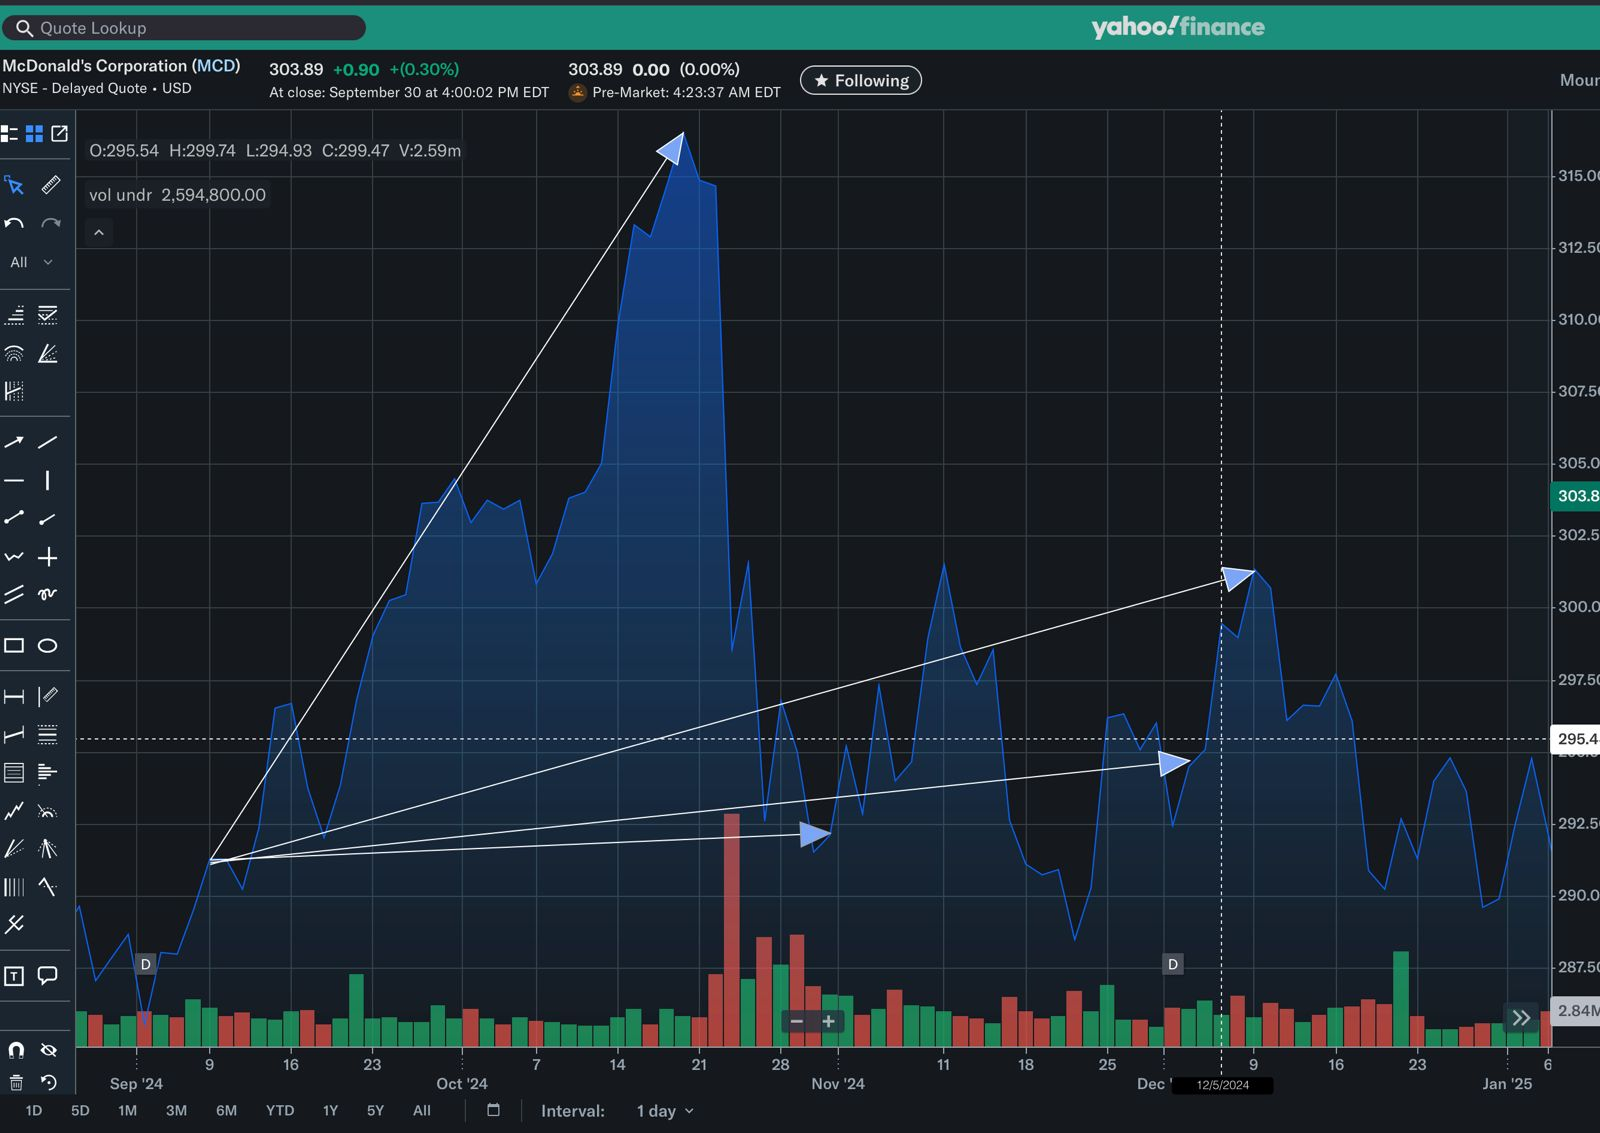
\includegraphics[width=0.85\linewidth]{mcdonalds.jpeg}
    \caption{McDonald's respective stock data}\cite{MCD}
    \label{fig:mcd}
\end{figure}
\FloatBarrier




\vspace{1.1cm}

\item \textbf{AMD} -- The narrator emphasized that the \textbf{artificial intelligence (AI) market} continues to expand rapidly.     While AMD cannot realistically challenge \textbf{NVIDIA’s market dominance}, 
    the overall growth of the sector indicates that AMD’s share of the \textbf{“AI Hype”} will also increase significantly \cite{cnbc}.
\vspace{0.3cm}

\textbf{Evaluation:} Although AMD’s stock declined sharply following the \textbf{April 2025 U.S. export control restrictions}, 
falling by approximately \textbf{37\%} \cite{AMD}, this was largely driven by investor fears of collapsing China GPU demand. 
However, the Q1 2025 financial report (released in \textbf{early May}) showed revenue decreased only slightly --- from 
\textbf{\$7.7 billion in Q4 2024}\cite{amdQ42024} to \textbf{\$7.44 billion in Q1 2025} \cite{amdQ1} (a drop of just \textbf{\$0.3 billion}). 
Expectations of a much steeper decline did not materialize. This reassured investors that AMD’s growth drivers --- particularly in \textbf{data center} and \textbf{AI-related segments} --- 
remained intact. As a result, long-term optimism around the AI market helped stabilize the stock, 
even though export restrictions and new customs regulations continued to affect revenues in the following 6--12 months. Moreover, the stock price had a steady increase to today, 11 \% increase between the dates 25.10.2024 - 10.02.2025, even surpassing the previous stock price while still suffering from the restrictions.\cite{AMD}
\newpage

\begin{figure}[H]
    \centering
    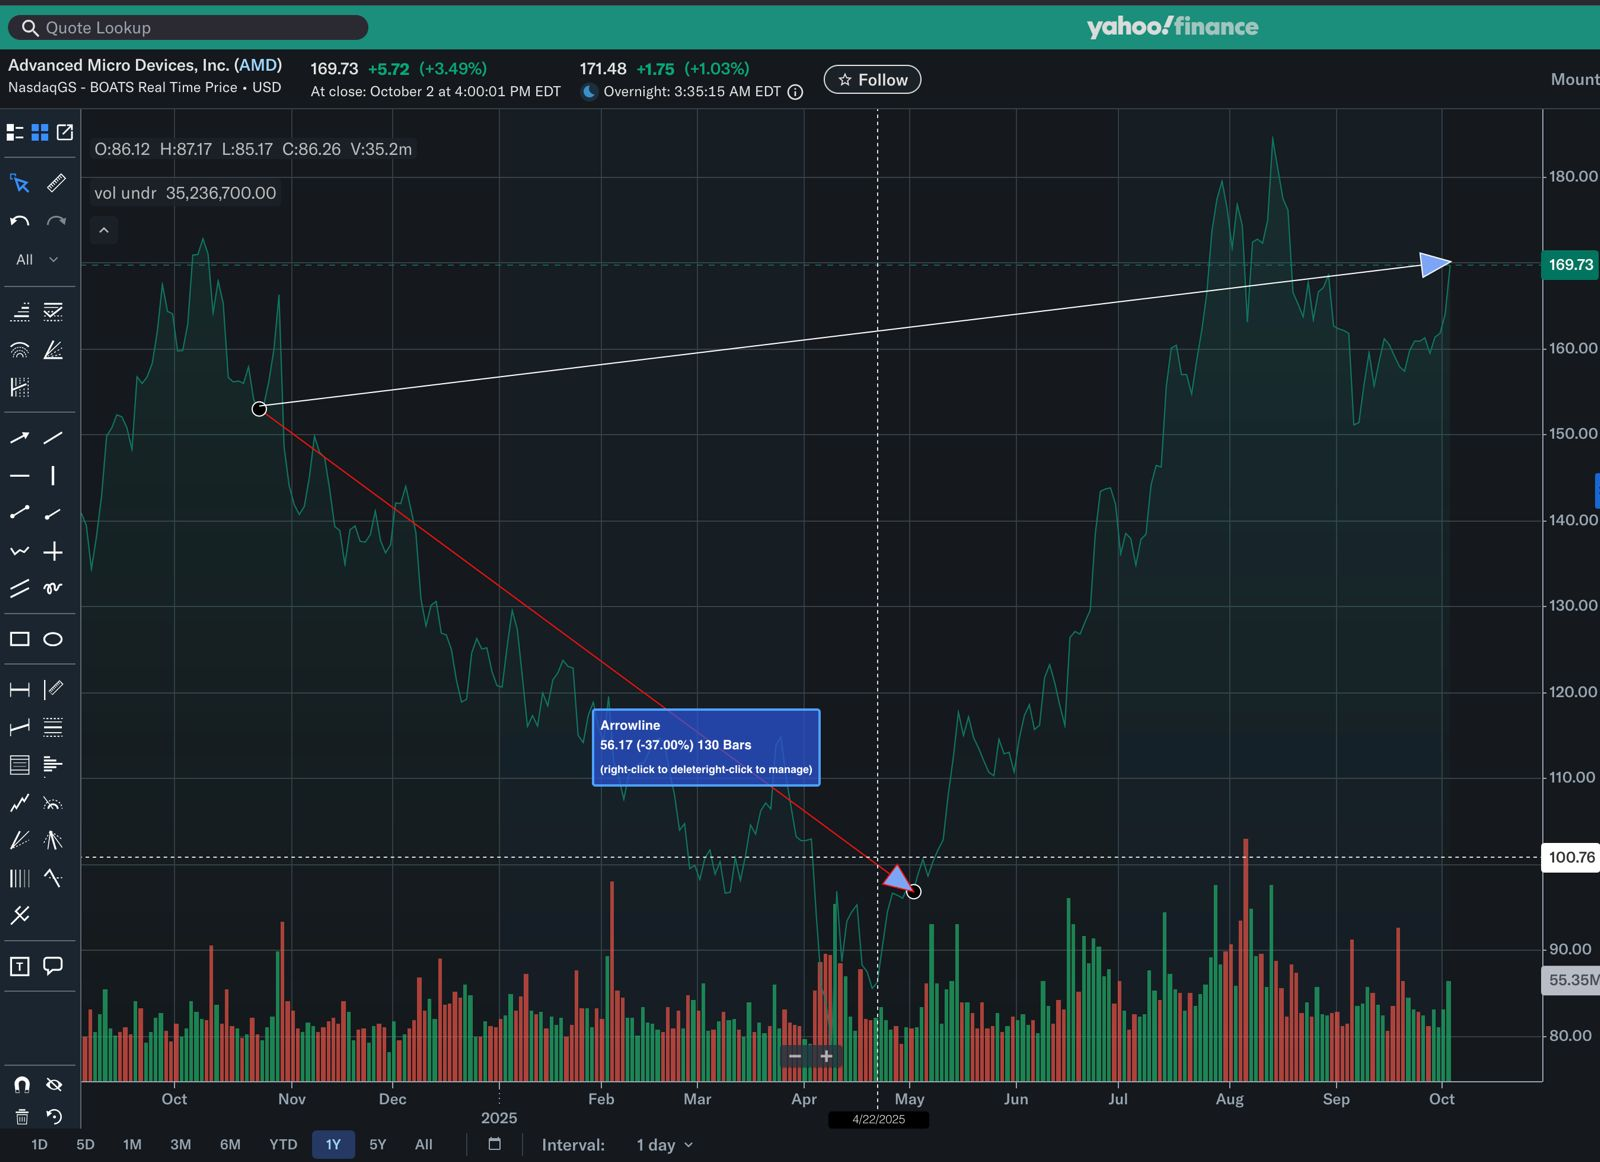
\includegraphics[width=0.85\linewidth]{amd.jpeg}
    \caption{AMD's respective stock data}\cite{AMD}
    \label{fig:amd}
\end{figure}
\FloatBarrier
\vspace{1.1cm}

    \item \textbf{UPS} -- Kramer emphasized that the main issue for UPS is \textbf{trust}. 
    Investors and analysts had lost confidence in management due to repeated underperformances, which left UPS in the era of \textbf{“show me stock”} \cite{cnbc}. 
    He also noted that the \textbf{brief port strike in late July 2024} gave UPS a short-term boost in its forwarding business, 
    even though global logistics were disrupted \cite{reutersUPS}. 
    Lastly, in Q2 2024 management forecasted a stronger second half, but investors doubted this guidance and sold off the stock \cite{UPS}. 
    In Q3 2024, UPS finally delivered stronger results, proving skeptics wrong \cite{UPS}. 
\vspace{0.3cm}

    \textbf{Evaluation:} The port strike impact was a temporary positive trigger, but as Kramer suggested, 
    it was essentially “artificial” and unsustainable. 
    UPS regained trust only after it showed real financial improvement in Q3, 
    demonstrating that short-term events can generate signals but lasting recovery depends on consistent performance.
\vspace{1.5cm}

\begin{figure}[H]
    \centering
    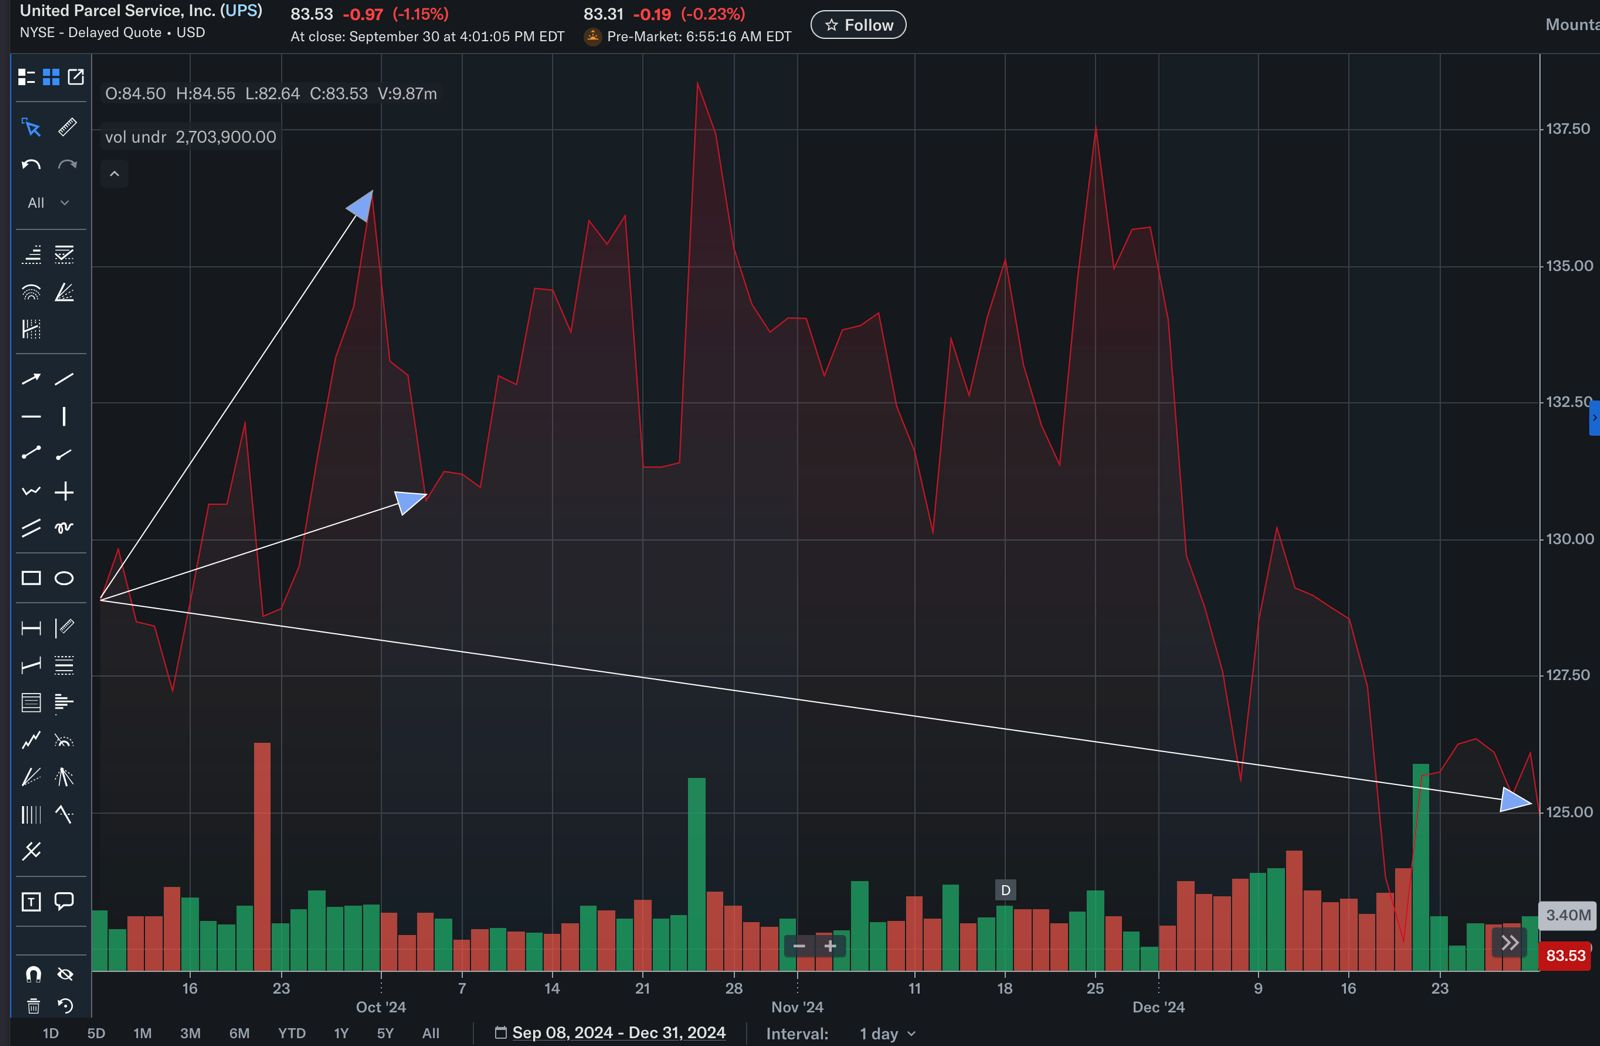
\includegraphics[width=0.85\linewidth]{upsd.jpeg}
    \caption{UPS's respective stock data\cite{UPS}}
    \label{fig:ups}
\end{figure}
\FloatBarrier
\vspace{1.1cm}

    \item \textbf{Tractor Supply} -- Kramer assessed Tractor Supply positively, 
    noting that the company delivered results largely in line with expectations. 
    However, since the stock had already risen by approximately \textbf{36\%}, 
    it was considered “hot,” and therefore dropped around \textbf{6\%} after earnings \cite{cnbc}. 
    He also interviewed CEO \textbf{Hal Lawton}, 
    who highlighted several themes: the viral popularity of the \textbf{TikTok “skeleton chicken”}, 
    the trend of \textbf{millennials relocating to rural areas}, 
    and the company’s growing \textbf{Neighbors Club membership program}, 
    strengthened by the acquisition of \textbf{Allivet} \cite{AllivetPR}.
\vspace{0.8cm}

     \textbf{Evaluation:} The viral TikTok “skeleton rooster” was a short-term phenomenon, unlikely to provide long-term value. 
    However, Tractor Supply’s membership-based foundation (\textbf{37+ million members}) 
    and demographic shifts toward rural living create sustainable revenue growth. 
    These fundamentals outweigh one-time viral boosts and suggest long-term positive signals. However, due to the seasonal nature of the company’s business and the influence of many other factors, it is not sufficient to evaluate performance based solely on this news.
\newpage


    \item \textbf{Tapestry - Capri acquisition} -- Kramer discussed the FTC lawsuit against Tapestry’s planned acquisition of Capri, 
    which Judge \textbf{Jennifer Rochon} ultimately blocked \cite{ftc}. 
\vspace{0.3cm}
    
\textbf{Evaluation for Capri:} The acquisition was announced on \textbf{10.08.2023} with an all-cash 
offer of \textbf{\$57 per share}, presenting a premium of about \textbf{59\%}. 
Capri’s stock immediately surged by nearly \textbf{55\%} \cite{CPRI}. 
When the FTC filed its lawsuit on \textbf{22.04.2024}, concerns intensified \cite{ftc}, 
and after Judge Rochon blocked the deal on \textbf{24.10.2024}, 
the stock collapsed by around \textbf{52\%} \cite{CPRI}. 
However, Capri’s stock had already fallen by about \textbf{42\%} during the year after the announcement \cite{CPRI}, 
showing how regulatory uncertainty eroded confidence well before the final ruling. 
This case illustrates how merger enthusiasm can quickly reverse under regulatory pressure.
\vspace{1.1cm}

\begin{figure}[H]
    \centering
    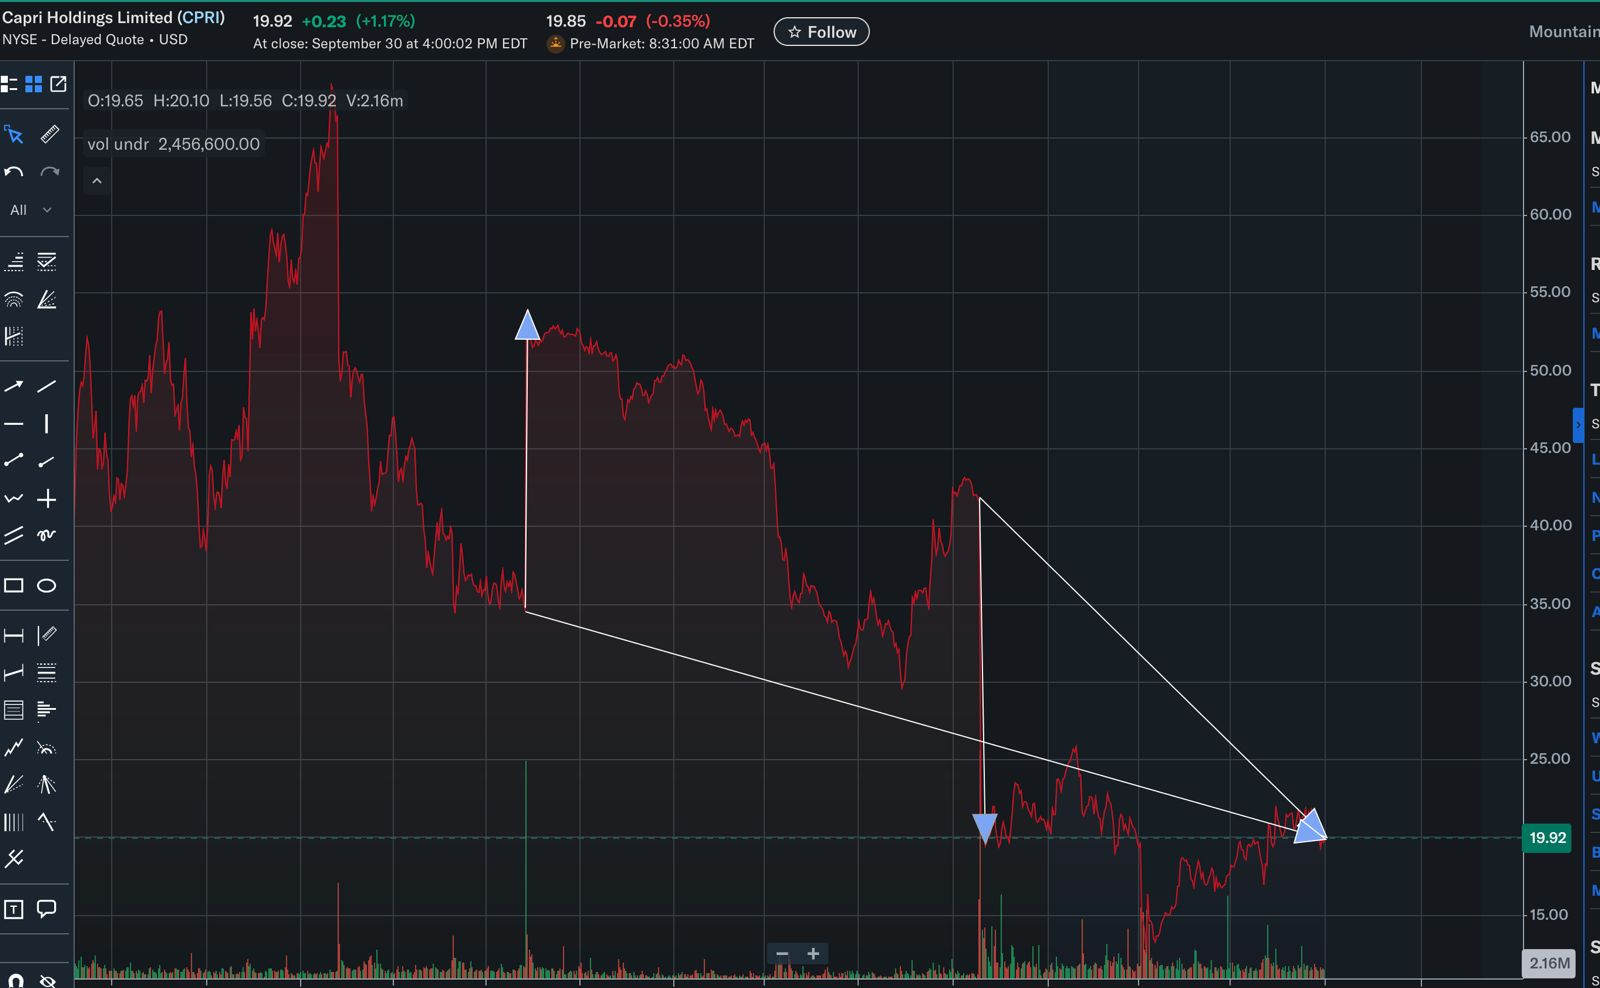
\includegraphics[width=0.85\linewidth]{capri.jpeg}
    \caption{Capri's respective stock data}\cite{CPRI}
    \label{fig:capri}
\end{figure}
\FloatBarrier

\vspace{1cm}
\textbf{Evaluation for Tapestry:} When the acquisition was announced, Tapestry faced the opposite reaction compared to Capri, with probably fewer long-term effects. Tapestry’s stock dropped by about \textbf{17\%} at the announcement but later rose by around \textbf{14\%} after the FTC canceled the deal.\cite{TPR} Between the announcement and the cancellation period, the stock had increased approximately \textbf{20\%}. Thus, the acquisition news had short-term effects on the stock price. During the period of uncertainty, investors may have gained confidence since there was a chance the deal would not happen. Finally, when it was canceled, even though Tapestry lost a major growth opportunity, investors were relieved that the heavy financial burden of the acquisition was removed, and in Forbes by Danziger , it is quoted as \textbf{"...it ultimately dodged a bullet by not taking on the problems at Capri}.\cite{forbesTapestry}


\begin{figure}[H]
    \centering
    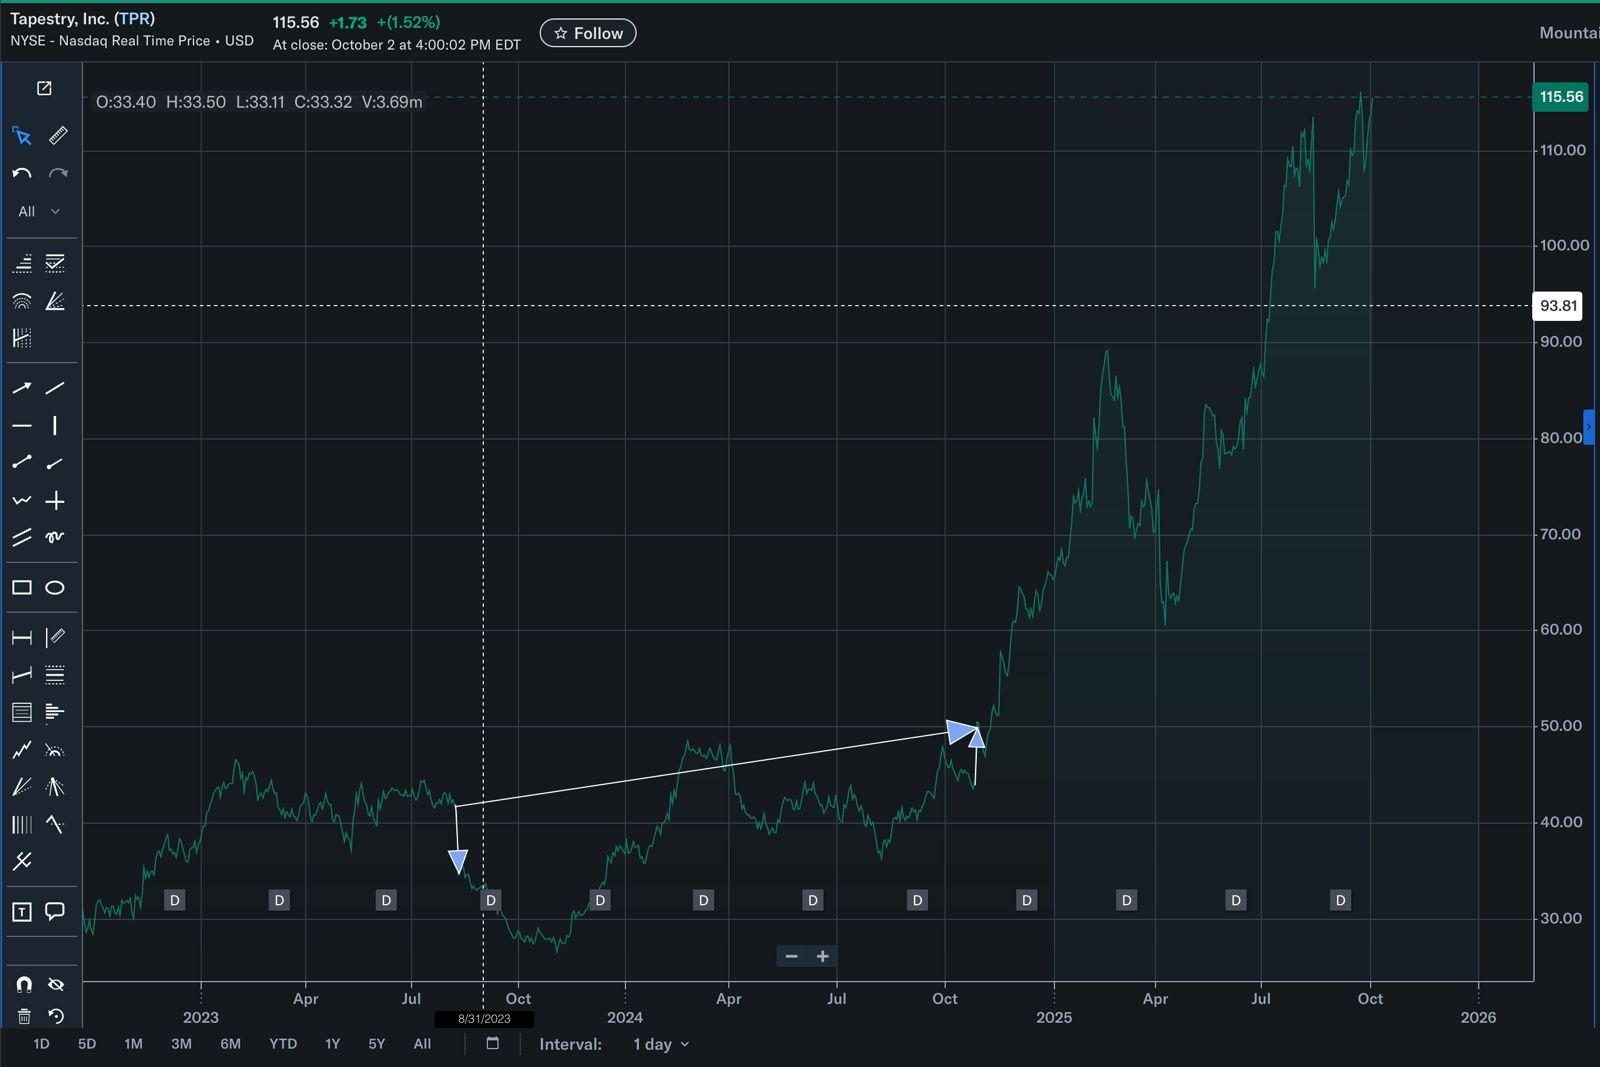
\includegraphics[width=0.85\linewidth]{Tapestry.jpeg}
    \caption{Tapestry's respective stock data}\cite{TPR}
    \label{fig:tapestry}
\end{figure}
\FloatBarrier




\end{itemize}

\vspace{1.1cm}

\section*{Conclusion}

\begin{quote}
Lastly, Kramer relates important events happening at the time with the stocks, which we used to examine further. For example: McDonald’s E. coli incident and its corresponding stock price; AMD’s export restrictions to China versus AI hype over time; UPS' event and its short-term effects; Tractor Supply’s long-term investments and how they could benefit the company; and the Tapestry–Capri acquisition and how it affected Capri \& Tapestry.  However,  even though these findings are not the only driver behind the stock market, as countless other factors affect the market, we attempted to highlight where a possible correlation may exist. 
\end{quote}
\newpage

\begin{thebibliography}{9}
\bibitem{amdQ1} Advanced Micro Devices. (2025, May 6).  
\textit{AMD Reports First Quarter 2025 Financial Results}. AMD Investor Relations.  
\url{https://ir.amd.com/news-events/press-releases/detail/1247/amd-reports-first-quarter-2025-financial-results}

\bibitem{amdQ42024} Advanced Micro Devices. (2025, February 4).  
\textit{AMD Reports Fourth Quarter and Full Year 2024 Financial Results}. AMD Investor Relations.  
\url{https://ir.amd.com/news-events/press-releases/detail/1236/amd-reports-fourth-quarter-and-full-year-2024-financial-results}

\bibitem{cnbc} CNBC. (2024, October 25).  
\textit{Mad Money with Jim Cramer}. [Video]. YouTube.  
\url{https://www.youtube.com/watch?v=1QRyRy0QUz0}

\bibitem{forbesTapestry} Danziger, P. (2024, November 15).  
\textit{Tapestry made the right decision to go it alone without Capri dragging it down}. Forbes.  
\url{https://www.forbes.com/sites/pamdanziger/2024/11/15/tapestry-made-the-right-decision-to-go-it-alone-without-capri-dragging-it-down/}

\bibitem{reutersUPS} Reuters. (2024, July 31).  
\textit{U.S. port strike hits global supply chains}.  
Retrieved from \url{https://www.reuters.com}

\bibitem{AllivetPR} Tractor Supply Company. (2024, October 24).  
\textit{Tractor Supply Company to Acquire Allivet, a Leading Online Pet Pharmacy}.  
Retrieved from \url{https://investors.tractorsupply.com}

\bibitem{ftc} U.S. Federal Trade Commission. (2024, April 22).  
\textit{FTC Moves to Block Tapestry’s \$8.5B Acquisition of Capri Holdings}.  
Retrieved from \url{https://www.ftc.gov/news-events/news/press-releases/2024/04/ftc-moves-block-tapestrys-acquisition-capri}

\bibitem{wikipedia} Wikipedia contributors. (2024).  
\textit{2024 McDonald’s E. coli outbreak}. In \textit{Wikipedia}.  
Retrieved from \url{https://en.wikipedia.org/wiki/2024_McDonald%27s_E._coli_outbreak}

\bibitem{AMD} Yahoo Finance. (2024–2025).  
\textit{Advanced Micro Devices, Inc. (AMD) Stock Historical Data}.  
Retrieved from \url{https://finance.yahoo.com/quote/AMD/history}

\bibitem{CPRI} Yahoo Finance. (2023–2024).  
\textit{Capri Holdings Limited (CPRI) Stock Historical Data}.  
Retrieved from \url{https://finance.yahoo.com/quote/CPRI/history}

\bibitem{MCD} Yahoo Finance. (2024).  
\textit{McDonald’s Corporation (MCD) Stock Historical Data}.  
Retrieved from \url{https://finance.yahoo.com/quote/MCD/history}

\bibitem{TPR} Yahoo Finance. (2024).  
\textit{Tapestry, Inc. (TPR) Stock Historical Data}.  
Retrieved from \url{https://finance.yahoo.com/quote/TPR/history}

\bibitem{UPS} Yahoo Finance. (2024).  
\textit{United Parcel Service, Inc. (UPS) Stock Historical Data}.  
Retrieved from \url{https://finance.yahoo.com/quote/UPS/history}

\end{thebibliography}
\end{document}